\documentclass{article}

\usepackage{graphicx}
\usepackage{hyperref}
\usepackage{tabularx}
\usepackage{alltt}
\usepackage{biblatex}
\usepackage{caption}

\usepackage[a4paper,total={6in, 8in}]{geometry}

\addbibresource{references.bib}

\graphicspath{{assets/}}

\newcolumntype{M}[1]{>{\centering\arraybackslash}m{#1}}
\newcommand{\IBS}[1] {\footnote{Itzik: #1}}

\begin{document}

%%%%%%%%%%%%%%%%%%%%%%%%%%%%%% TITLE %%%%%%%%%%%%%%%%%%%%%%%%%%%%%%%%%%%%%%
\title{PARALLEL A-STAR}

\tableofcontents

\author{
    Salvatore Licata \\
    Lorenzo Ferro \\
    Alessandro Zamparutti
}

\date{
    August 2022
}

\maketitle

%%%%%%%%%%%%%%%%%%%%%%%%%%%%%% Sections %%%%%%%%%%%%%%%%%%%%%%%%%%%%%%%%%%%%%%

\section{Introduction}
\label{Sec:intro}

Implementation of the A-Star algorithm both parallel and sequential versions on large and weighted benchmark graphs.
Study on performance and comparison between the 2 implementations.

The project implies:
\begin{itemize}
    \item reading of large weighted benchmark graphs
    \item run of A-Star parallel, sequential and standard Djkstra algorithm
    \item comparison considering computation time and memory usage
\end{itemize}
\section{Graph reading}
\label{Sec:reading}

Starting from a .map file (standard format for maps representation, using ascii characters to represent walls and passable terrain)
the \verb|graph_generator.py| python script is able to create a .txt with the format required by our A* implementation. \\
In the benchmark section we have:
\begin{itemize}
	\item huge-graphs: graphs with millions of nodes, used for comparisons on large dimensions
	\item maze: graph with a small number of solutions (few path available from a point to another)
	\item street-maps: true city grid maps with different sizes
	\item small-graphs: generated by us used for testing
\end{itemize}
The weight of the edges can be randomized by the script in order to raise the level of difficulty in finding a path (all the grids have only edges with unitary weight).
\\
The file is processed sequentially, creating all the nodes first and then the edges.

\section{Basic structures}
\label{Sec:basic_structures}

The project started by implementing all the basic structures needed by the algorithm, which are as generic as possible to encourage reuse and are dynamically allocated and implemented using lists to have no static limitations.
\\
Each structure has a create function for allocation and a destroy one for disallocation of the memory.

\subsection{hash table}
\label{hash_table}

It is implemented with multiplicative modular method with golden ratio:

\begin{equation}
    golden\_ratio = (\sqrt{5} - 1)/2
\end{equation}
\begin{equation}
    P = 8191
\end{equation}
\begin{equation}
    hash(key, module) = ((key*golden\_ratio)\%P)\%module
\end{equation}

The structure re-allocates itself when reaches the 3/4 of the maximum capacity, in case of collisions it concatenates the elements in a list (keeps in the first place the last inserted item).

\subsection{heap}
\label{heap}

It uses a hash table for faster addressing and it is used as a priority queue, with the possibility to have MAX or MIN priority as first element.

\subsection{queue}

Generic list with head and tail pointers to an item. FIFO queue with head extraction and tail insertion.

\subsection{stack}
\label{stack}

LIFO implementation with both insertion and extraction from the head.

\subsection{graph}

Generic Graph with possibility to be UNDIRECTED or DIRECTED, has a pointer to a generic data (useful when creating the graph from different domains such as 2D or 3D maps). A custom function can be passed as a parameter to properly read all the additional data. \\
Each vertex has a true\_cost, which is the cost of the path from the start to that specific vertex, and a heuristic\_cost, an exstimation of the cost from that node to the destination node.
The graph also contains a hash table of all the nodes used to search efficiently (a good improvement in the graph generation).

\subsection{message queue}
\label{message_queue}

It is composed by an array of queues, as long as the number of threads of the program.
The receive and send methods are protected by a mutex to avoid race conditions, and receive an Id to send/receive a message to/from a specific queue. 
It also has a function to check if all the queues are empty, which is used in the parallel A* algorithm for the terminate detection.

\section{A-Star Implementation}
\label{Sec:implementation}

The A-Star algorithm is based on the use of a heuristic function which exstimates the cost from a point to a destination node.

Both implementations are based on two set, the OPEN and the CLOSE one. The first is implemented using a priority queue (our heap \ref{heap}) and contains nodes that have been discovered but not expanded yet, the other one with a hash table (\ref{hash_table}) and contains node that have been expanded.

All vertex contains a link to a parent vertex which is used to keep trace of the path found by the algorithm, at the end the solution is inserted in a stack (\ref{stack}) pushing from the goal node and going backward.

\subsection{Sequential}

Starting from pseudo-code \cite{bibParAstar}

\begin{alltt}
    1 Initialize OPEN to \{s_0\};
    2 while OPEN \(\neq\) 0; do
    3 Get and remove from OPEN a node n with a smallest f(n);
    4 Add n to CLOSED;
    5 if n is a goal node then
    6   Return solution path from \(s_0\) to n;
    7 for every successor n' of n do
    8   $g_1$ = g(n) + c(n; \(n'\));
    9   if n' \(\in\) CLOSED then
    10      if g_1 < g(n') then
    11          Remove n' from CLOSED and add it to OPEN;
    12      else
    13          Continue;
    14  else
    15      if n' \(\notin\) OPEN then
    16          Add $n'$ to OPEN;
    17      else if $g_1$ \(\geq\) g($n'$) then
    18          Continue;
    19  Set g($n'$) = g_1;
    20  Set f($n'$) = g($n'$) + h($n'$);
    21  Set parent($n'$) = n;
    22 Return failure (no path exists);
\end{alltt}

Where
\begin{itemize}
    \item $s_0$ : is the starting node
    \item $g(n)$ : is the cost of the best known path from $s_0$ to $n$
    \item $h(n)$ : is the heuristic function
    \item $f(n)$ : is the sum $g(n) + h(n)$, used in the OPEN set to calculate the priority
\end{itemize}

\subsection{Parallel}

Implementation of the decentralized AStar algorithm, where each thread has its own CLOSED and OPEN set, when a thread discovers a neighbouring node choses the thread that will expand it and sends a message to it.
\\
When a thread find a solution, it compares the cost with the global one and if it has a lower cost, it just change the cost with the new one (the global cost is protected with a lock).

\subsubsection{Pseudo-code}

Starting from pseudo-code \cite{bibParAstar}

\begin{alltt}
    1 Initialize OPENp for each thread p;
    2 Initialize incumbent.cost = \(\infty\);
    3 Add s0 to OPENComputeRecipient(s0);
    4 In parallel, on each thread p, execute 5-31;
    5 while TerminateDetection() do
    6   while BUFFERp \(\neq\) 0 ; do
    7       Get and remove from BUFFERp a triplet (n0; g1; n);
    8       if n0 2 CLOSEDp then
    9           if g1 < g(n0) then
    10              Remove n0 from CLOSEDp and add it to OPENp;
    11             else
    12                  Continue;
    13      else
    14          if n0 =2 OPENp then
    15              Add n0 to OPENp;
    16          else if g1  g(n0) then
    17              Continue;
    18      Set g(n0) = g1;
    19      Set f(n0) = g(n0) + h(n0);
    20      Set parent(n0) = n;
    21  if OPENp = ; or Smallest f(n) value of n 2 OPENp \(\geq\) incumbent.cost then
    22      Continue;
    23  Get and remove from OPENp a node n with a smallest f(n);
    24  Add n to CLOSEDp;
    25  if n is a goal node then
    26      if path cost from s0 to n < incumbent:cost then
    27          incumbent = path from s0 to n;
    28          incumbent.cost = path cost from s0 to n;
    29  for every successor n0 of n do
    30      Set g1 = g(n) + c(n; n0);
    31      Add (n0; g1; n) to BUFFER ComputeRecipient(n);
    32 if incumbent:cost = 1 then
    33  Return failure (no path exists);
    34 else
    35  Return solution path from s0 to n;
\end{alltt}

Where
\begin{itemize}
    \item $BUFFER$ : structure used for thread communication (\ref{thread_buf})
    \item $incumbent$ : the shared best known path
    \item $TerminateDetection$ : function to check if the path search is completed \ref{terminate}
    \item $ComputeRecipient$ : function that choses the thread that will expand the node (\ref{compute_reci})
\end{itemize}

\subsubsection{Compute recipient}
\label{compute_reci}

A Function that is able to map the nodeId into a thread identifier, and which is used to decide to which thread send a message with the node to expand.
This function can considerably change the performance of the algorithm.
\\ We provided two different implementation:
\\
The basic module is the simplest one and it is computed as: \\
$node\_id \; \% \;  number\_of\_threads$
\\
A more efficient function, but still simple to implement, is the multiplicative hashing computed as \cite{bibVideoMulHash}: \\
$ h(node\_id) =((a*node\_id \; + \; b) \; \% \; p) \; \% \; number\_of\_threads $  
\\ where:
\begin{itemize}
    \item $p$: prime large number (we used INT\_MAX =  $ 2^{31}-1 $)
    \item $a$: random integer [1,p-1]
    \item $b$: random integer [0,p-1]
\end{itemize}


\subsubsection{Thread communication}
\label{thread_buf}

A message queue \ref{message_queue} structure is used to allows threads to communicate: a thread compute the recipient and send a message using the thread destination with the node and cost. 

\subsubsection{Terminate condition}
\label{terminate}

When a thread has its OPEN set empty or there isn't elements that will improve the cost of the path, it sets its termination\_flag.
A thread waits on his condition variable only if it has no message pending and its termination\_flag is set, if all other threads are waiting the program terminates instead.
When a thread sends a message to another one it signal its condition variable in order to waking it up. 

\begin{alltt}
    1 lock mutex
    2 while termination_flags[this_thread] and
    BUFFER(this_thread) = 0 AND not program_terminated
    3   if(counter \( \geq \) n_threads - 1 AND all buffer empty
    4       program_terminated = 1
    5       signal all condition variables
    6   else
    7       counter++
    8       wait on condition variable of this_thread
    9       counter--
    10 unlock mutex
    11 if program_terminated
    12   return true
    13 else
    14   return false
\end{alltt}

Where
\begin{itemize}
    \item $termination\_flags$: array of flags setted by a thread when the OPEN set is empty or does not has any node with a minor cost then the actual path
    \item $program\_terminated$: flag setted by last thread awake when it detects the termination of the program
    \item $counter$: counter of sleeping threads
    \item $mutex$: global mutex to protect all condition variables
    \item $BUFFER$: message queue of each thread
\end{itemize}


\section{Experimental evaluation}
\label{Sec:experimental-eval}

Here we report the result of the tests executed to compare the performance between the sequential and parallel version of the A-Star implementation.\\
To test the parallel A* algorithm we changed the number of threads and the function used to compute the recipient (\ref{compute_reci}). \\
All the tests are performed on a Linux environment.

\subsection{Time performance}


\subsubsection{Grid Milan}
The graph generated from the grid of Milan (1024x1024) has around 800k nodes and has random generated weights to increase the difficulty to find the path with the best cost.

\begin{center}
    
    \begin{minipage}[b]{0.3\textwidth}

            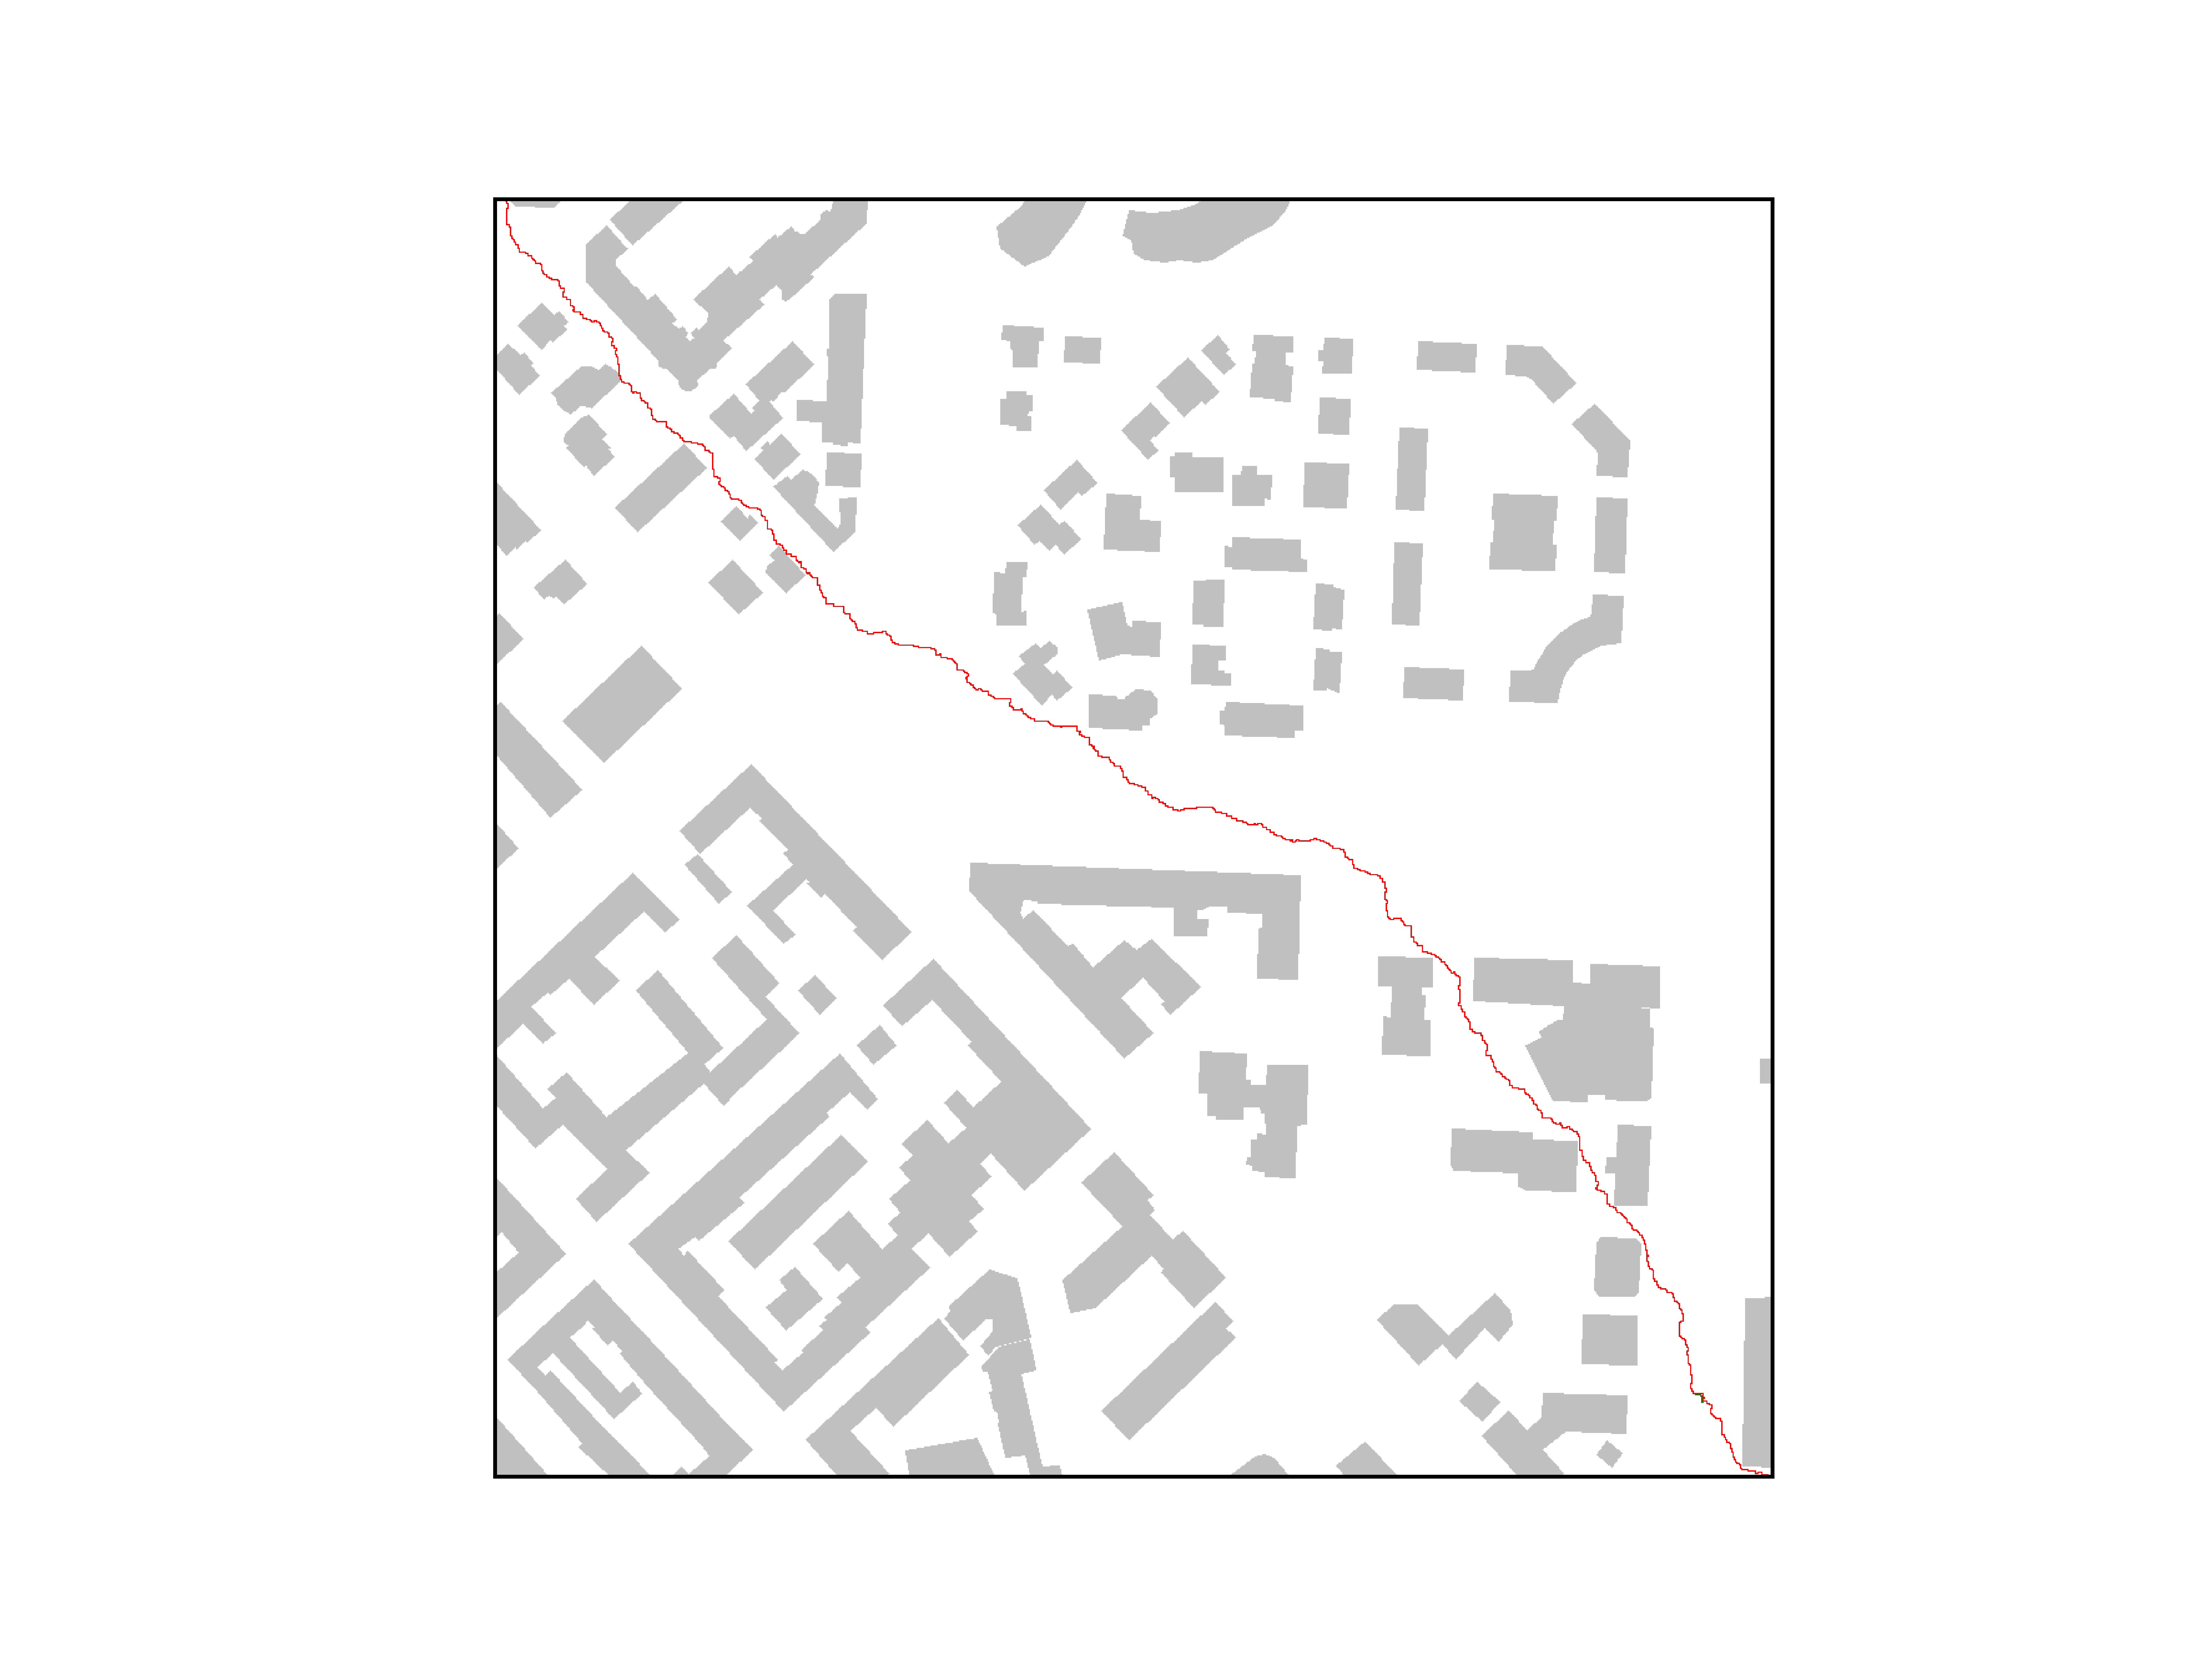
\includegraphics[scale=0.5]{gridMilan.png}
            \captionof{figure}{Milan map with path found}
            \label{Milan-grid}
        
    \end{minipage}%
    \begin{minipage}[b]{0.6\textwidth}
        
            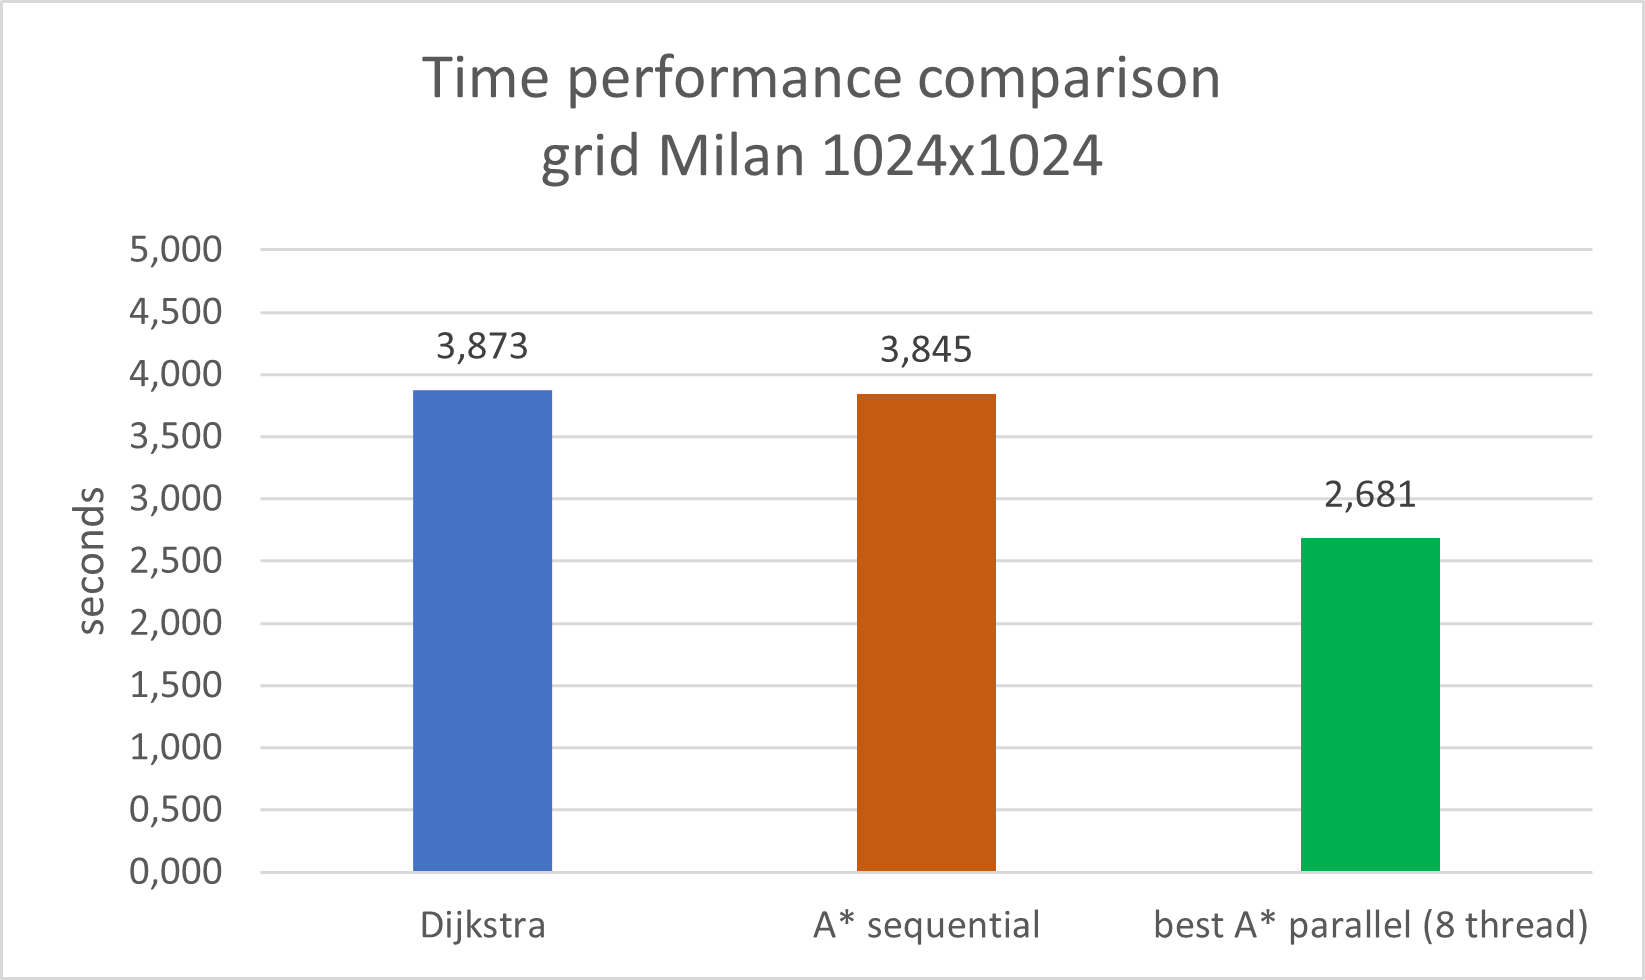
\includegraphics[scale=0.7]{milanComparison.png}
            \captionof{figure}{Performance comparison on different algorithms}
            \label{Milan-comp}
    \end{minipage}
    
\end{center}


\begin{figure}
    \centering
    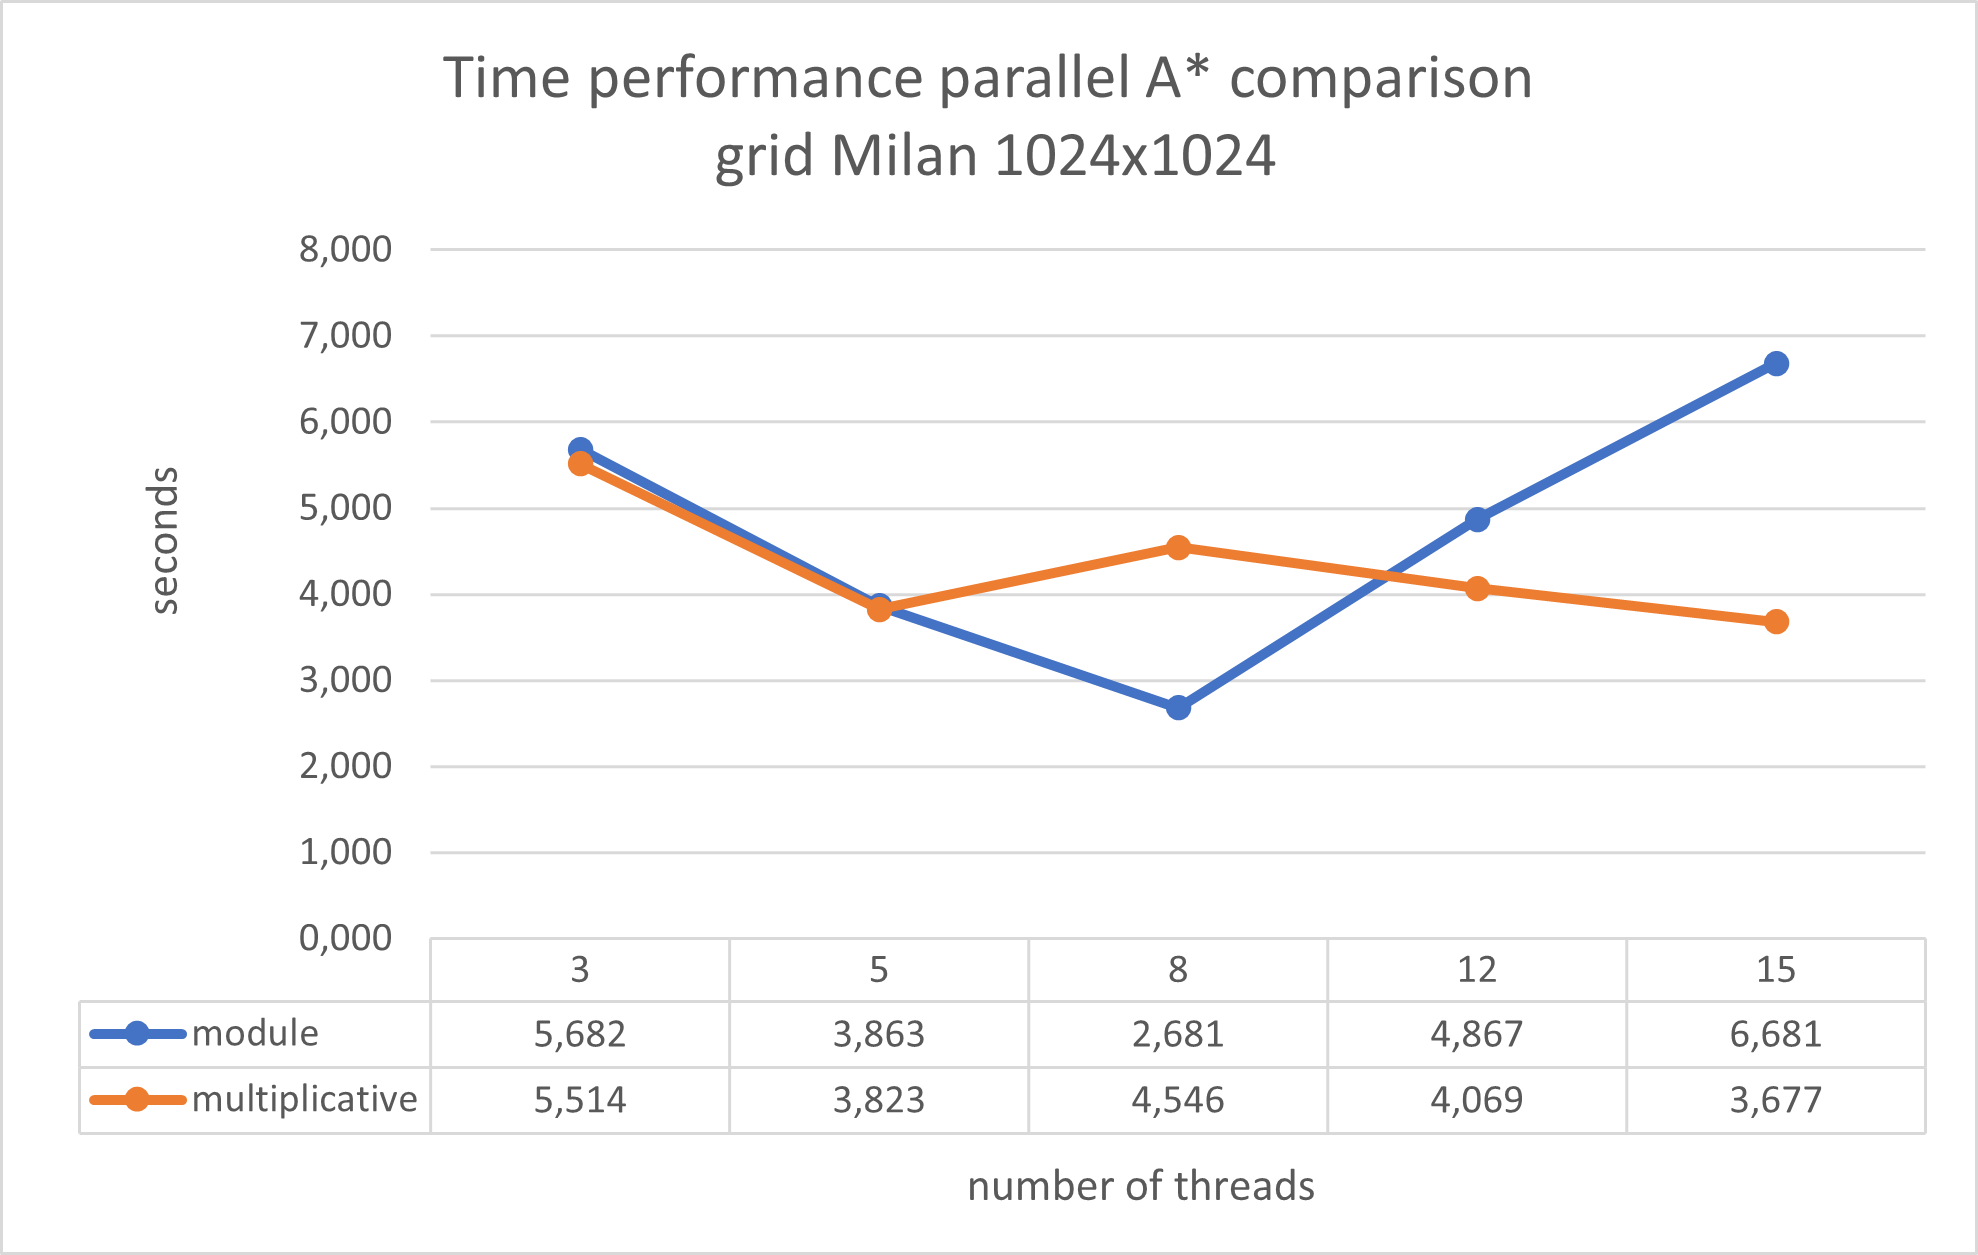
\includegraphics[scale=0.7]{milanParComparison.png}
    \caption{Performance comparison on different thread number and compute recipient function}
    \label{Milan-par-comp}
\end{figure}


Looking at Figure \ref{Milan-comp}, and taking into account that we chose the most efficient number of threads for parallel A*,
we can notice a better performance compared to the sequential A* and the Dijkstra algorithms. 
To find the best result we tried the parallel A* changing the number of threads and the compute recipient function:
the Figure \ref{Milan-par-comp} shows all the experimental results of the tests.
\\
Comparing the two compute recipient functions (simple module and multiplicative hash)
on this relative small graph, it can be observed that when runnig with limited number of threads the performance are similar.
When increasing the level of parallelism the performances are no loger comparable, and the algorithm with the multiplicative hash function is faster.


\subsubsection{Large Map}

To test more our algorithms we used larger graphs, always with random weights, with about 4 Millions nodes.

\begin{figure}
    \centering
    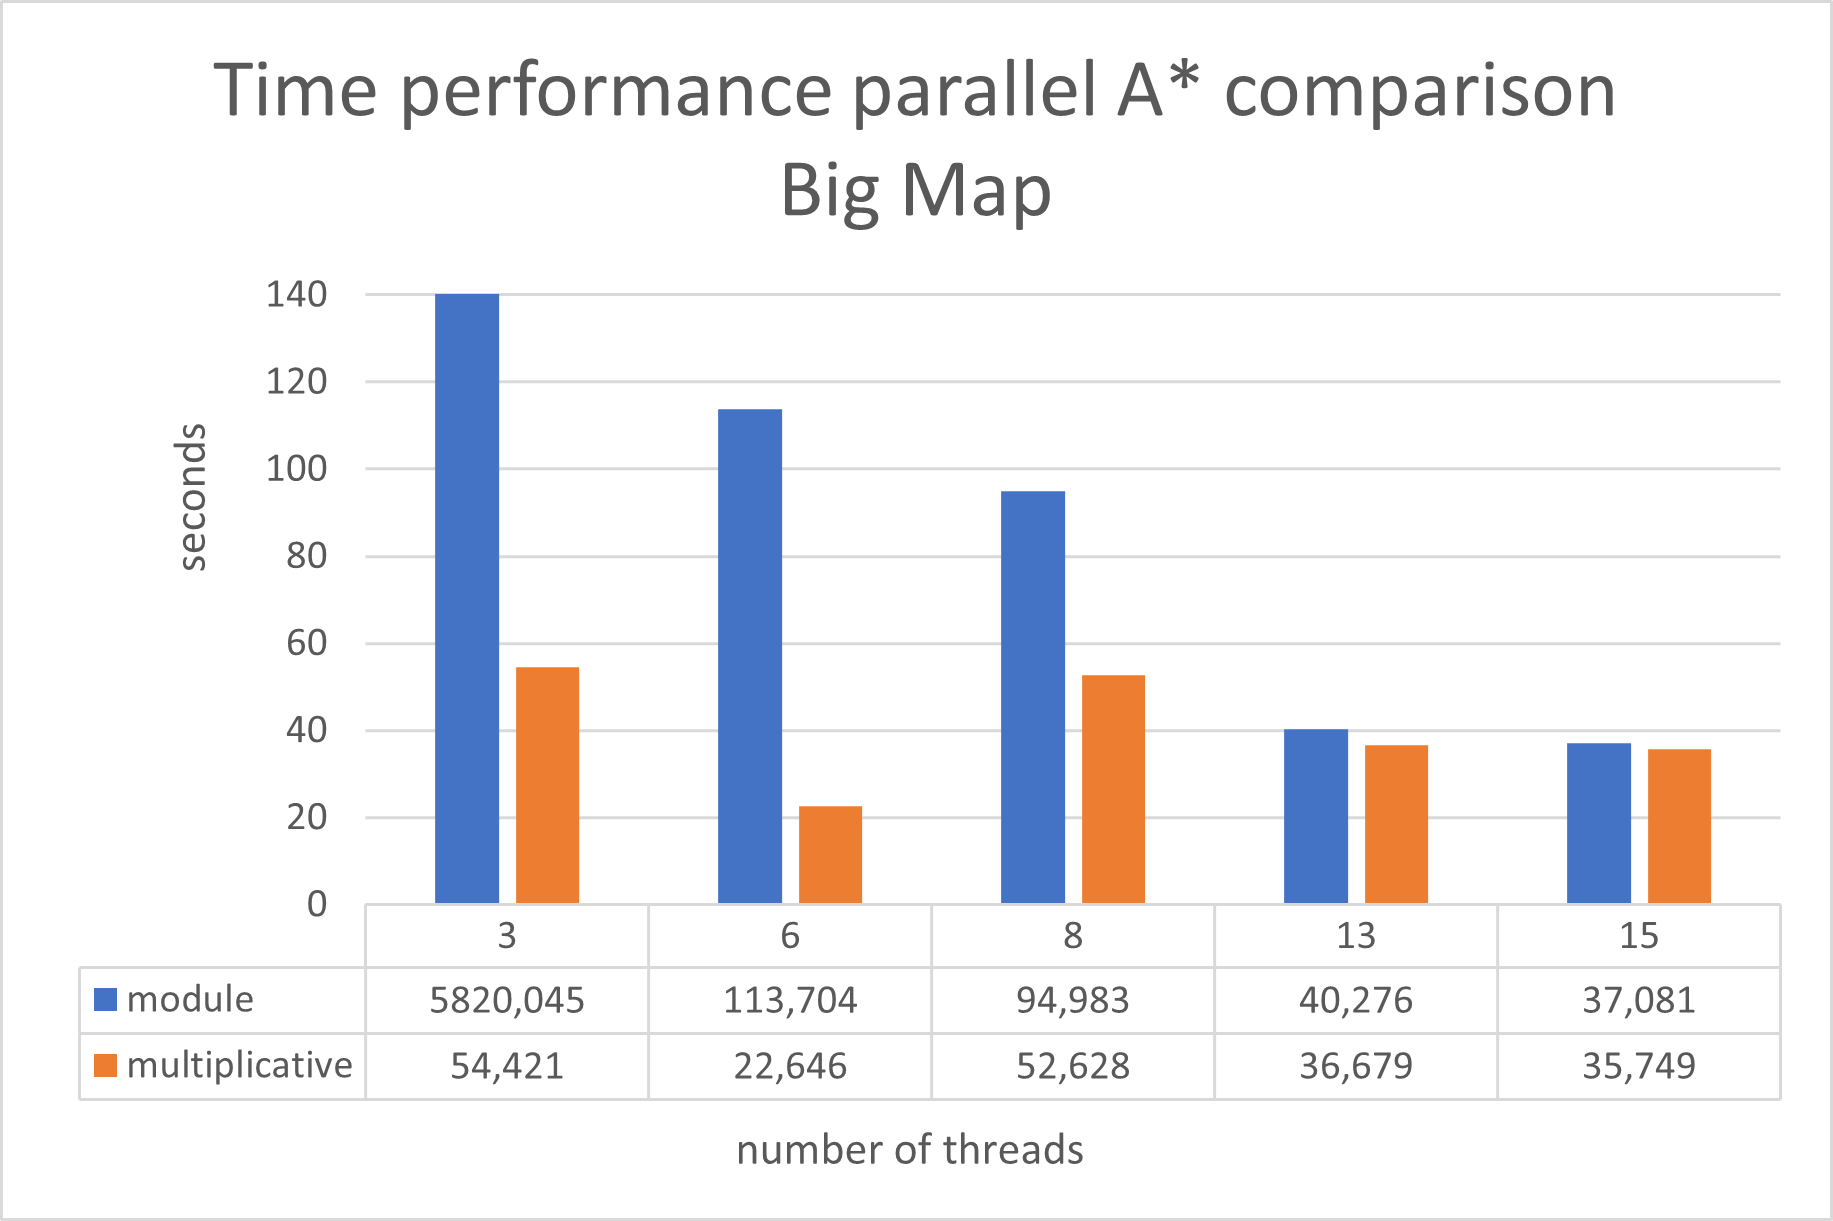
\includegraphics[scale=0.7]{mapParComparison.png}
    \label{Map-par-comp}
    
    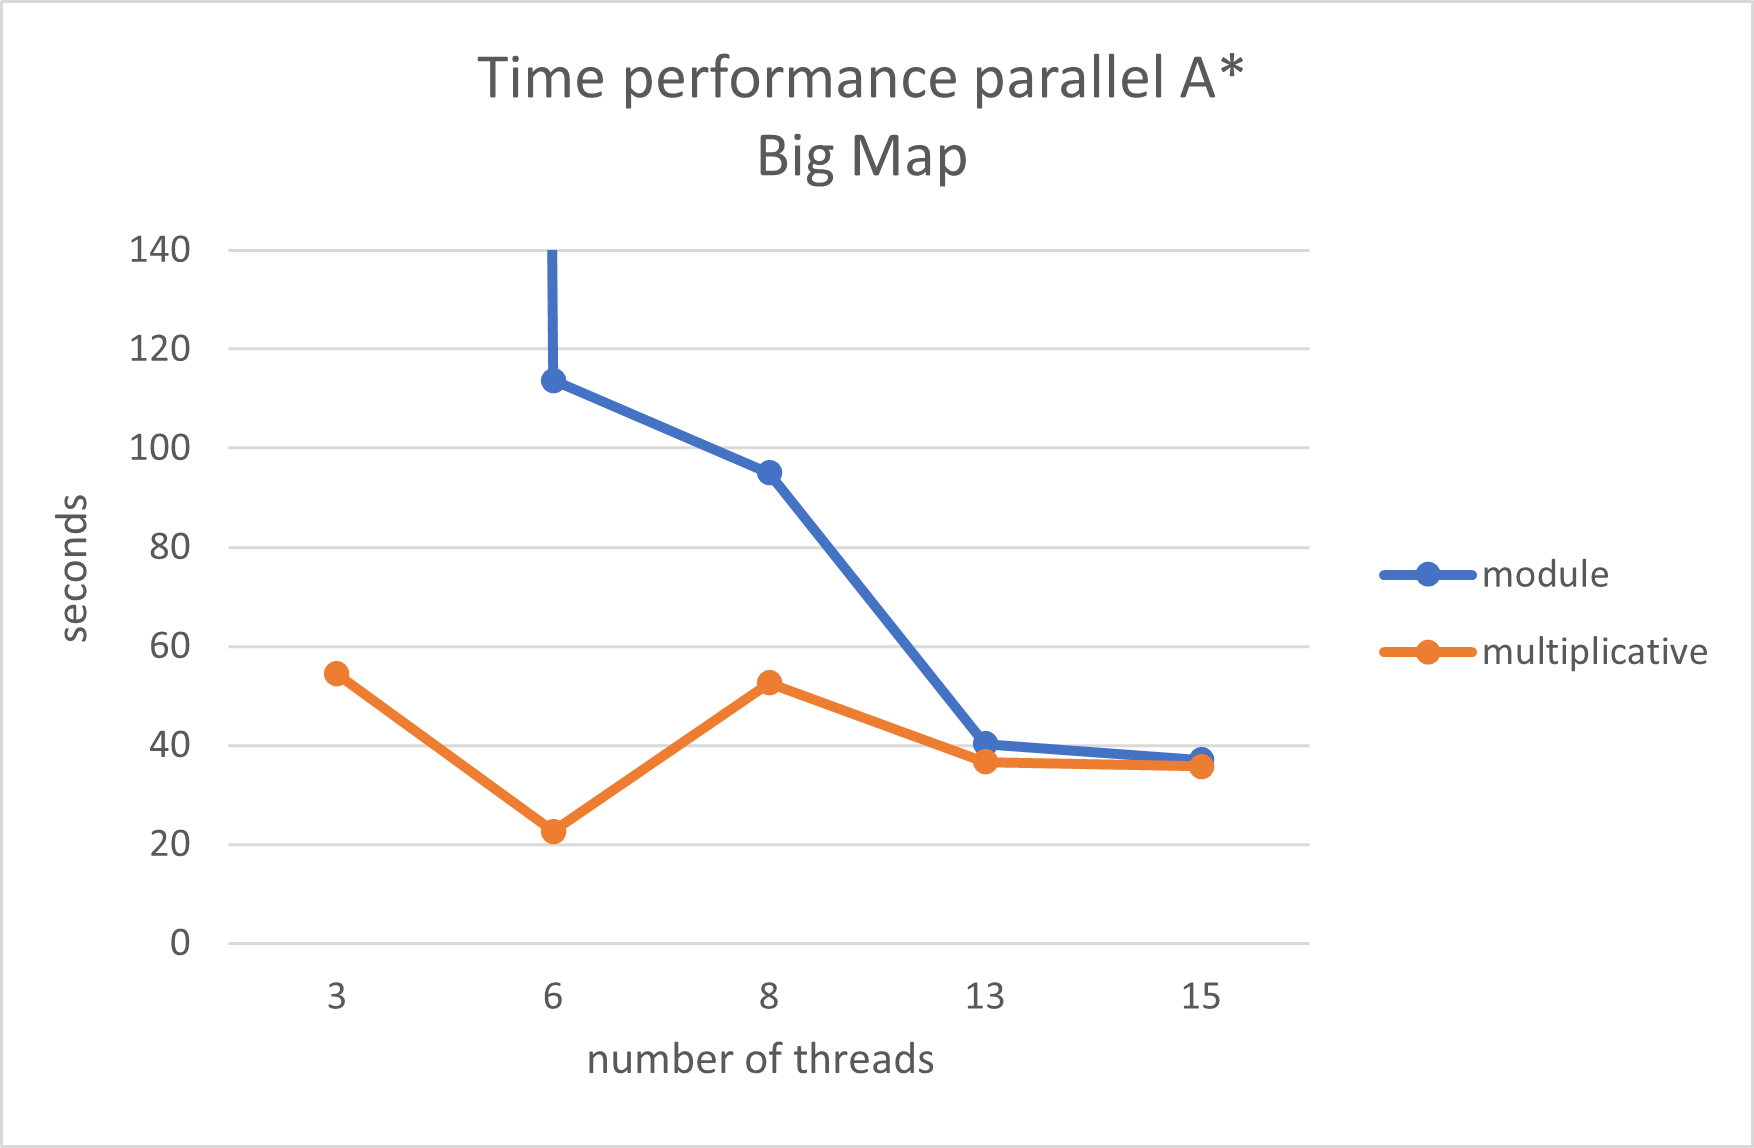
\includegraphics[scale=0.7]{mapParComparisonLines.png}
    \label{Map-par-comp-lines}
    \caption{Performance comparison on different thread number and compute recipient function}
\end{figure}


By looking at the results on Figure \ref{Map-par-comp}, it can be observed that the multiplicative hash function is more stable when changing the number of threads.
For small level of parallelism (eg. 3 threads) the module hash needs almost two hours to found the correct path, while exploring and revisiting a large number of nodes.
The seconds needed to find a path decreses considerably with the increasing of the number of threads, but for some value (mostly even values of threads eg. 12), the time to converge to a result greaty increases again.
The multiplicative hash instead, has generally better performances, but we found some limits on the number of threads (again even values from 16 onwards) beyond which the time increases.


\subsection{memory occupation}

To track the memory occupation we used the Valgrind-Massif tool which is a heap profiler. It measures how much heap memory the program uses: this includes both the useful space,
and the extra bytes allocated for book-keeping and alignment purposes.
\\
The graph generated shows the memory occupation on specific time snapshots. The X axis indicates the bytes allocated/deallocated on the heap and stack(s), while the Y axis shows the actual memory occupation on that specific snapshot.


\begin{figure}
    \centering
    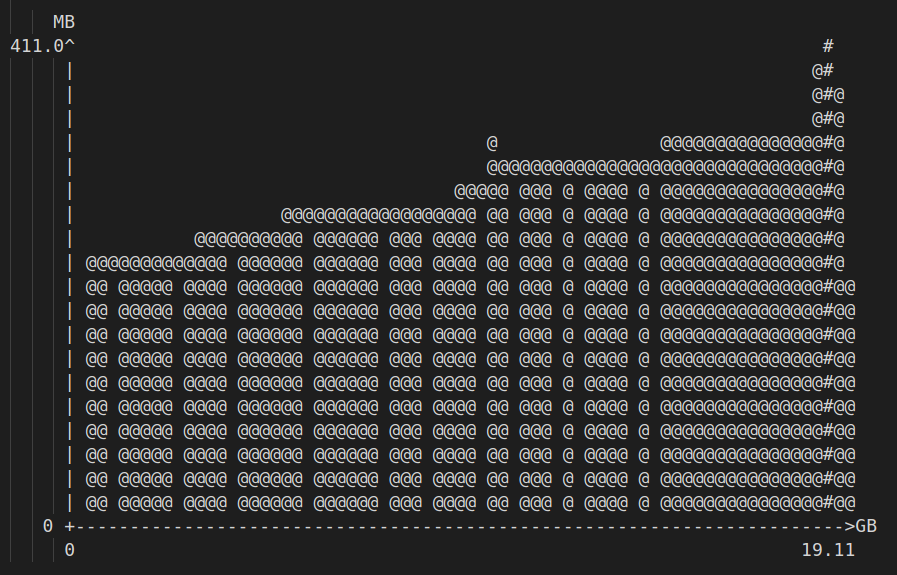
\includegraphics[scale=0.4]{mem_milan_par.png}
    \caption{Memory occupation of parallel A* with Milan grid}
    \label{mem-par-milan}
\end{figure}


\begin{figure}
    \centering
    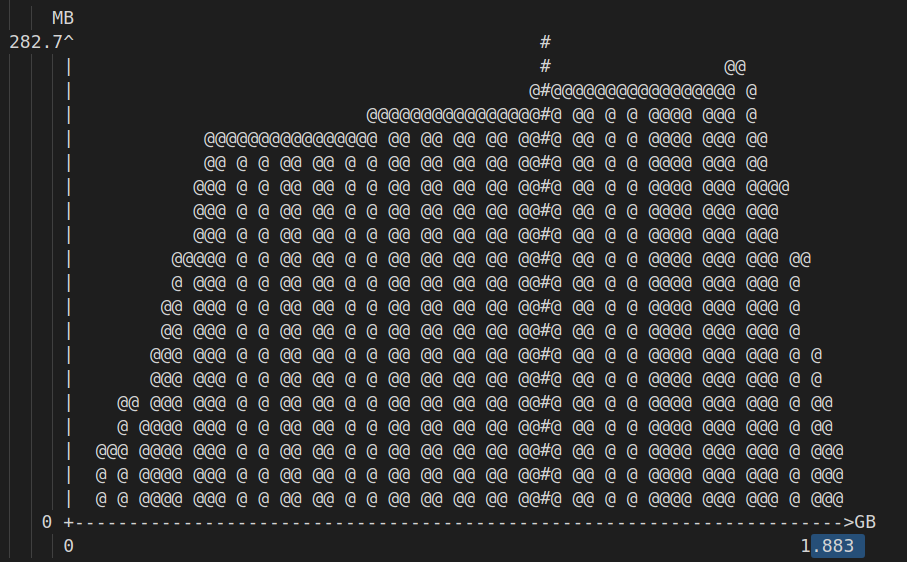
\includegraphics[scale=0.4]{mem_milan_seq.png}
    \caption{Memory occupation of sequential A* with Milan grid}
    \label{mem-seq-milan}
\end{figure}

As expected the occupation of the sequential A* is lower, since it has only one OPEN and CLOSED sets and it does not need to allocate additional structures for threads communication and synchronization.
It can be also noticed the difference between the sum of all the allocation made by the two algorithms.



\begin{figure}
    \centering
    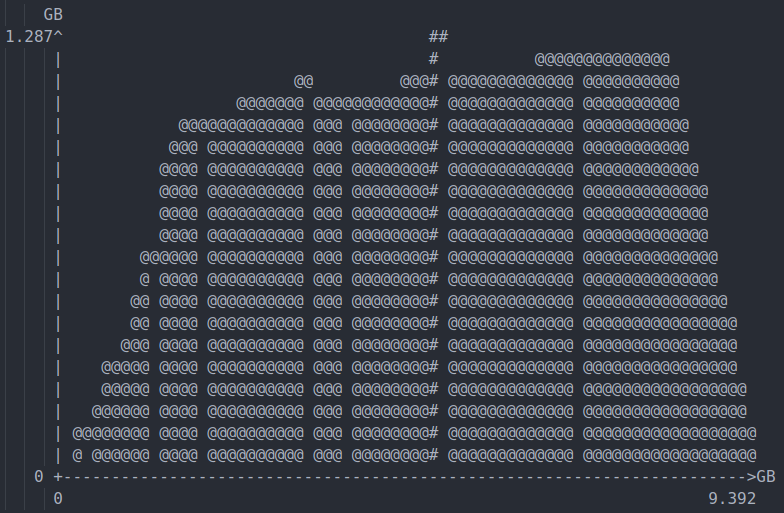
\includegraphics[scale=0.4]{mem_map_seq.png}
    \caption{Memory occupation of sequential A* with large map}
    \label{mem-seq-map}
\end{figure}

\begin{figure}
    \centering
    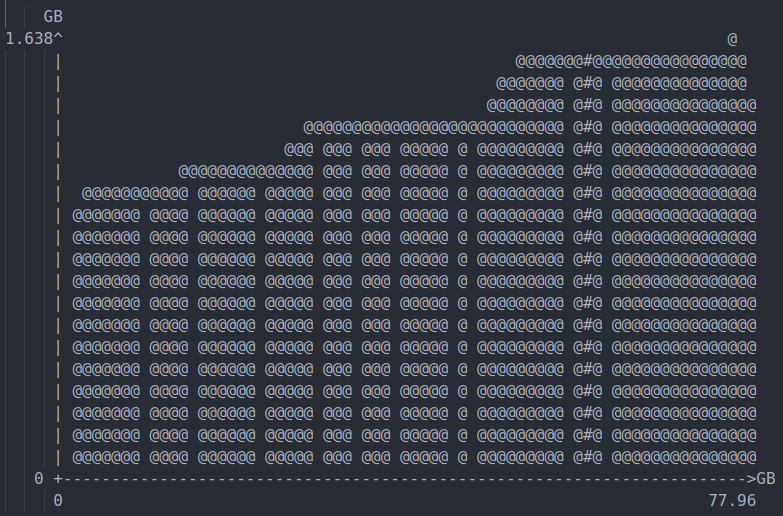
\includegraphics[scale=0.4]{mem_map_par.png}
    \caption{Memory occupation of parallel A* with large map}
    \label{mem-par-map}
\end{figure}


To ensure that are not memory leak we used an option of the Valgrind tool which keep track of all heap blocks issued in response to calls to malloc.
As shown by the the Figure \ref{mem-leak-milan} the algorithm does not have any memory leakage.

\begin{figure}
    \centering
    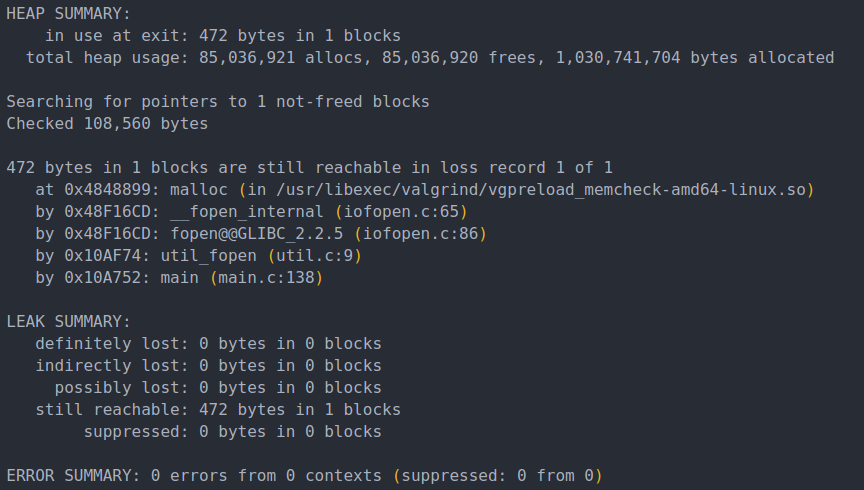
\includegraphics[scale=0.4]{mem_leak_report.png}
    \caption{Valgrind output of memory leak of parallel A* with Milan grid}
    \label{mem-leak-milan}
\end{figure}



\input{sections/pos_enhancement.tex}

\nocite{*}
\printbibliography


\end{document}

